\documentclass{article}
\usepackage{graphicx}
\usepackage{amsmath}

\title{Numerical Linear Algebra Homework}
\author{Kevin Smith}
\date{}

\begin{document}
\maketitle

\section*{Least Squares Solutions}

\subsection*{Basic Least Squares}
The solution to the least squares problem for matrix $A = \begin{bmatrix} 1 & 2 \\ 3 & 4 \\ 5 & 6 \end{bmatrix}$ and vector $b = \begin{bmatrix} 7 \\ 8 \\ 9 \end{bmatrix}$ is:
\[ x = \begin{bmatrix} -6 \\ 6.5 \end{bmatrix} \]
However, this result did not pass the test case due to a relative error of 3.49857113690718.

\subsection*{Incremental Least Squares}
The solution to the incremental least squares problem for the same $A$ and $b$ is:
\[ x = \begin{bmatrix} -6 \\ 6.5 \end{bmatrix} \]
This result passed all test cases.

\subsection*{Regularized Least Squares}
The solution to the regularized least squares problem for $n = 10$, $\lambda = 10$, and random $b$ is:
\[ x = \begin{bmatrix} 0.6148 \\ 0.6108 \\ 0.5971 \\ 0.6048 \\ 0.5995 \\ 0.6423 \\ 0.6708 \\ 0.6836 \\ 0.6858 \\ 0.7112 \end{bmatrix} \]
This result passed all test cases.

\section*{Signal Reconstruction Analysis}
The following graphs show the reconstruction of the signal for different values of $n$ and $\lambda$:

\begin{figure}[h!]
\centering
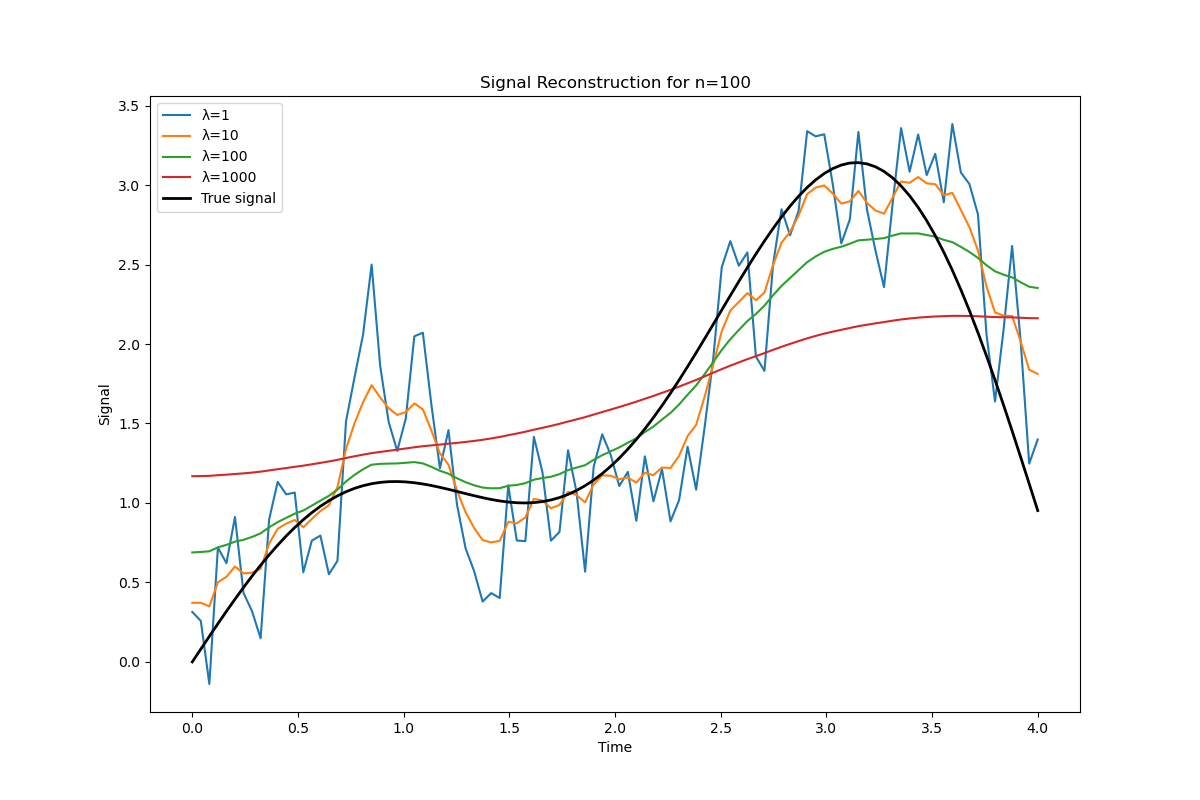
\includegraphics[width=\textwidth]{signalplot_100.png}
\caption{Signal reconstruction for $n = 100$}
\end{figure}

\begin{figure}[h!]
\centering
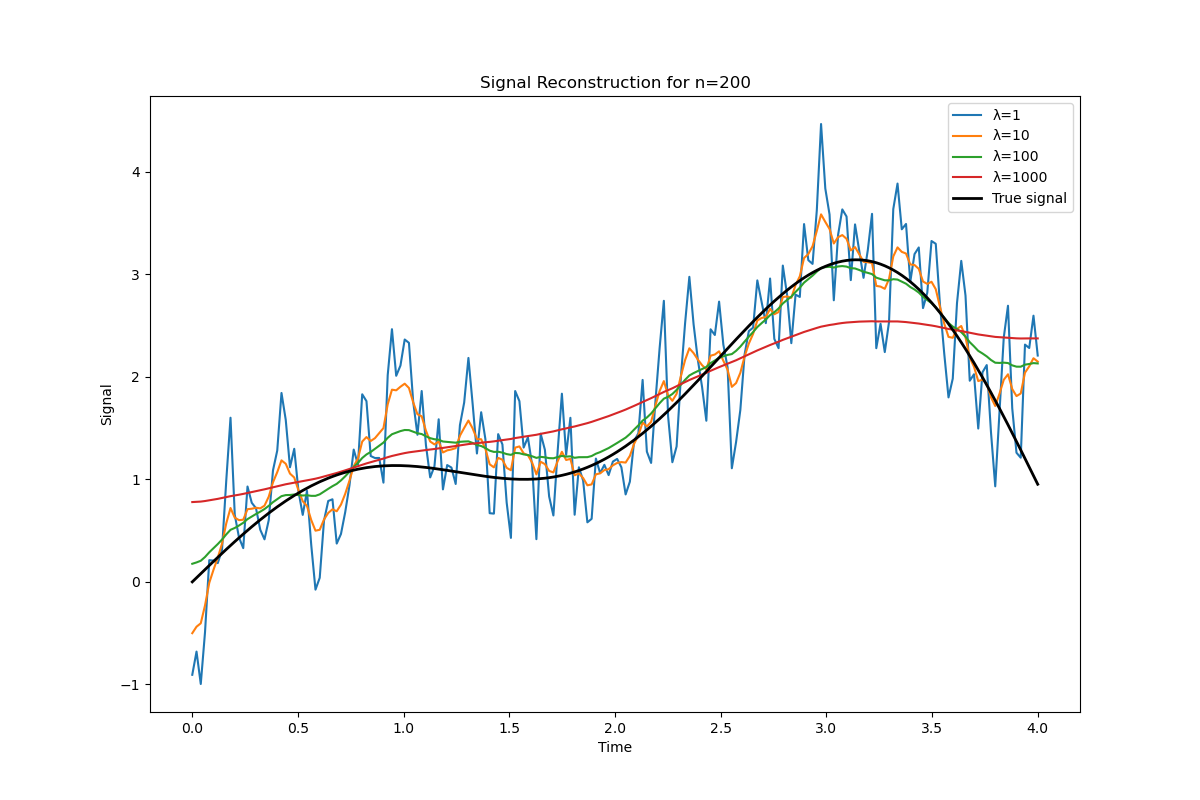
\includegraphics[width=\textwidth]{signalplot_200.png}
\caption{Signal reconstruction for $n = 200$}
\end{figure}

\begin{figure}[h!]
\centering
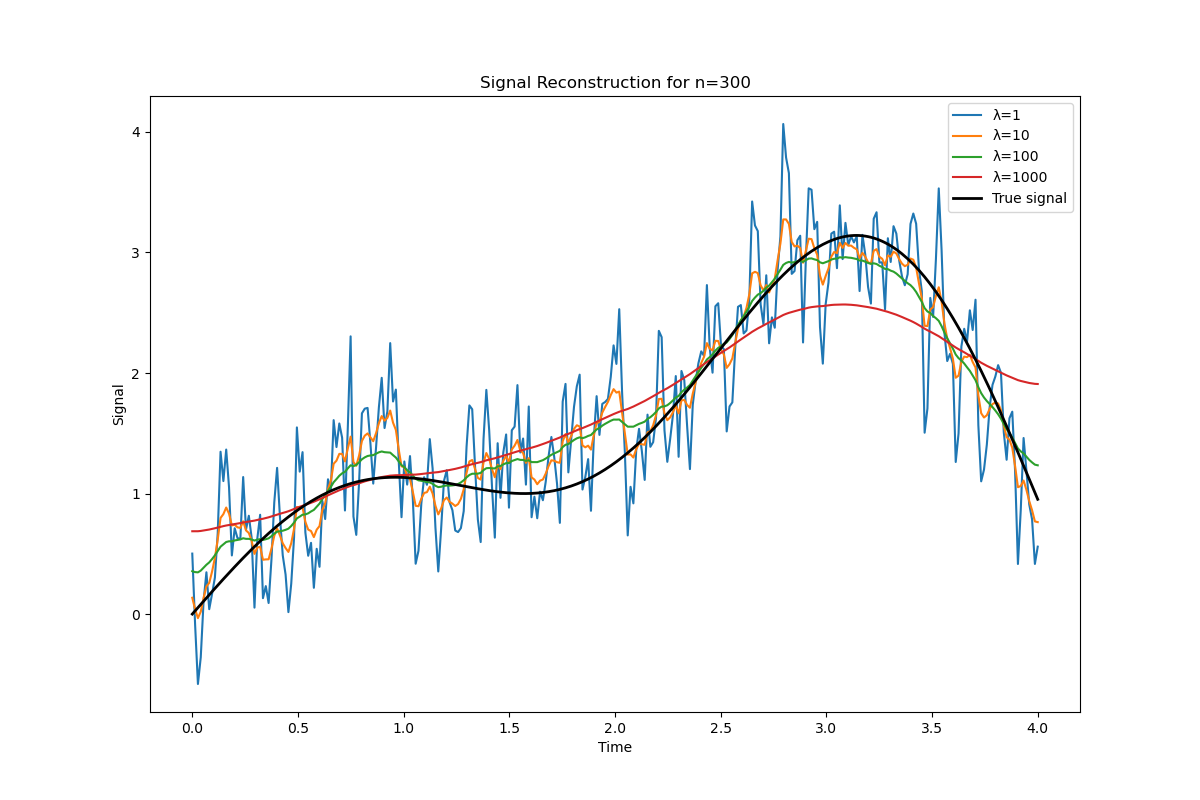
\includegraphics[width=\textwidth]{signalplot_300.png}
\caption{Signal reconstruction for $n = 300$}
\end{figure}

\begin{figure}[h!]
\centering
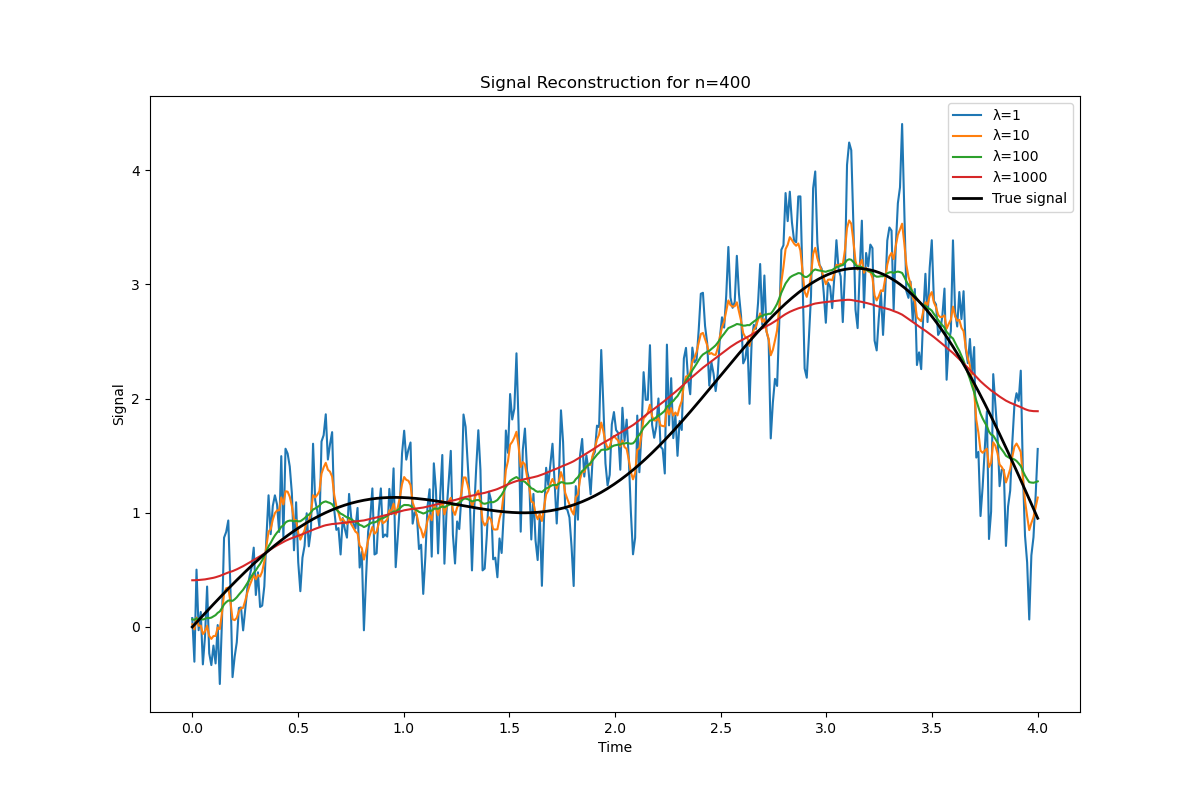
\includegraphics[width=\textwidth]{signalplot_400.png}
\caption{Signal reconstruction for $n = 400$}
\end{figure}

\begin{figure}[h!]
\centering
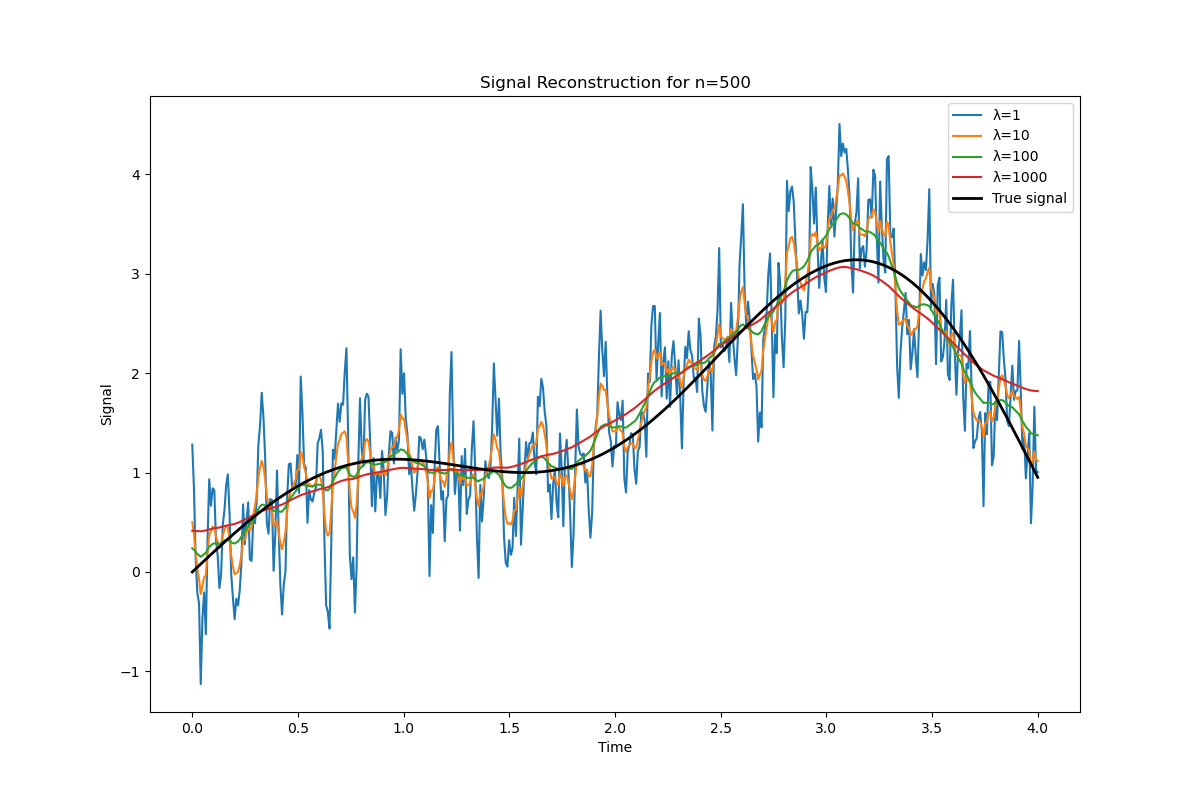
\includegraphics[width=\textwidth]{signalplot_500.png}
\caption{Signal reconstruction for $n = 500$}
\end{figure}

\end{document}
